\documentclass{my_paper}
\usepackage{ctex}
\usepackage[textwidth=444bp,vmargin=2.5cm]{geometry}%设置页边距
\usepackage{array} %主要是增加列样式选项
\usepackage[dvipsnames]{xcolor}%颜色宏包
\usepackage{graphicx}%图片宏包
\usepackage{amsmath}%公式宏包
\usepackage[T1]{fontenc}    
\usepackage{newtxtext, newtxmath}  %两种使用Times New Roman 字体的方法
\usepackage{subfigure}
\usepackage { gensymb }
% 打°符号\degree
\usepackage{listings}
% 代码
\usepackage{listings}

\lstset{language=python,                    %Python语法高亮
    linewidth=0.9\linewidth,            %列表list宽度
    %basicstyle=\ttfamily,              %tt无法显示空格
    commentstyle=\color{commentcolor},  %注释颜色
    keywordstyle=\color{keywordcolor},  %关键词颜色
    stringstyle=\color{stringcolor},    %字符串颜色
    %showspaces=true,                   %显示空格
    numbers=left,                       %行数显示在左侧
    numberstyle=\tiny\emptyaccsupp,     %行数数字格式
    numbersep=5pt,                      %数字间隔
    frame=single,                       %加框
    framerule=0pt,                      %不划线
    escapeinside=@@,                    %逃逸标志
    emptylines=1,                       %
    xleftmargin=0em,                    %list左边距
    % backgroundcolor=\color{backcolor},  %列表背景色
    tabsize=4,                          %制表符长度为4个字符
    gobble=4                            %忽略每行代码前4个字符
    }

\usepackage{color} %red, green, blue, yellow, cyan, magenta, black, white
\definecolor{mygreen}{RGB}{28,172,0} % color values Red, Green, Blue
\definecolor{mylilas}{RGB}{170,55,241}
\lstset{language=Matlab,%
    %basicstyle=\color{red},
    breaklines=true,%
    morekeywords={matlab2tikz},
    keywordstyle=\color{blue},%
    morekeywords=[2]{1}, keywordstyle=[2]{\color{black}},
    identifierstyle=\color{black},%
    stringstyle=\color{mylilas},
    commentstyle=\color{mygreen},%
    showstringspaces=false,%without this there will be a symbol in the places where there is a space
    numbers=left,%
    numberstyle={\tiny \color{black}},% size of the numbers
    numbersep=9pt, % this defines how far the numbers are from the text
    emph=[1]{for,end,break},emphstyle=[1]\color{red}, %some words to emphasise
    %emph=[2]{word1,word2}, emphstyle=[2]{style},    
}
\begin{document}

%----------- 中文摘要 ----------
\newpage
\begin{center}
    \fontsize{15.75pt}{0}\heiti 多仓库自卸车实时调度策略
\end{center}
尊敬的经理先生:

经过我们团队长达三天的研究与测试,对您的仓库和车辆的调度策略有些建议,希望能够帮助到您。

这套系统主要实现了借用摄像机对单个仓库或多个仓库用大小各一辆自卸车的实时卸料安排。

首先我们介绍摄像头的安装位置,为了达到“实时”调度的目的,摄像头位置的选择对我们模型的精度十分重要,我们需要矿料的正视图和俯视图,对于单个仓库我们只需安装2个摄像头,一个位于仓库正前方,另一个位于仓库的顶部。而对于多个仓库,可以在能够分辨清楚矿料边界和高度的前提下减少摄像头的数量,比如可以将2个摄像头安装在两个仓库的中间位置(一个在前方一个在顶部),这样六个仓库我们只需要3组,即6个摄像头。

单个仓库的位置如下图所示:

\begin {figure}[h]
\centering % 居中显示
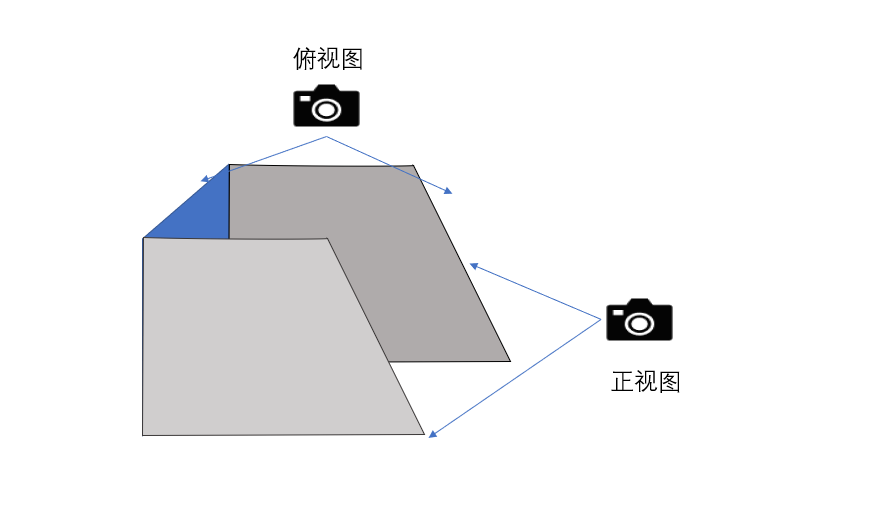
\includegraphics[width=\textwidth]{camera_lay.png}
\end {figure}
 
然后是单个仓库车辆卸货的调度安排,我们能够根据矿料的性质和您拥有的自卸车的参数模拟出常见的几种堆放结果,如平地自由堆放、背面靠墙堆放、在已有的堆上堆放,我们后续也会使用这几种基本情况作为调配的依据。我们先根据摄像头拍摄得到矿料的边界,进而利用背靠墙堆放的模拟结果进行边界匹配。考虑到卸货车只能将矿料卸载到矿料的边界,且最终的仓库上限是一条直线,所以我们不断地维持目前物料最平整的堆放方式。我们用背靠墙的模拟来近似每次填放后的局部物料变化,因此我们采用图形相似的方法来计算最适合填补物料的边界位置和最适用的自卸车类型。在图形匹配算法中,我们用最能近似在已有堆料前提下继续堆放的方式——靠墙堆放的模拟结果,作为目标形状,并依据自卸车的参数和矿料的安息角计算出货箱能够深入堆料的最大深度,以此确定形状的内边界,最后采用离散化变线为点得到一个可遍历的有限结果集合,进而从中选择形状相似度最佳的位置和车型,得到一个最佳方案后,我们再使用计算机来进行模拟,以降低我们的近似误差。

最后是多个仓库的联合调度,因为仓库最主要的是存储,所以我们优先使仓库存储尽量多的矿料,再考虑用更短的时间完成矿料堆放。结合实际,矿料的价值和需求量、仓库的存储成本不同,我们对多个仓库还设置了优先级的堆放策略。就是先求出各个仓库的最佳车型和位置,因为自卸车的资源有限,需要凭借优先级,完成不平等的车型分配,就是优先满足您认为重要的仓库的需求。

这篇建模的数据均有较权威的数据和理论支撑,数据均从相关官网搜的,物理模型的建立参考了多篇权威科学论文,并且我们对模型还经行了多次测试和修改,并用计算机实现了具体例子的处理,所以我们的模型和算法拥有很高的合理性和实用性。

在此模型中,凡是会随基本情况,如车辆参数、矿料参数都设为了变量值,十分方便修改,因此此模型也拥有较广泛的适用性。

\begin{flushright}
    数模实验小组

    2022年4月24日
\end{flushright}


\newpage
\begin{center}
\lunwenbiaoti

\vspace{2ex}
\zhaiyao
\end{center}


矿料仓库广泛存在于建筑、化工与农业等领域,由于矿料形状不定,仓库环境危险,研究自动化管理矿料仓库的方法具有重要的现实意义。本文采用边缘检测方法估计仓库中矿料体积,利用元胞自动机理论模拟矿料坍塌行为,使用形状匹配方法确定自卸车种类及位置,具有良好的效果。

针对问题一:我们利用两个不同方位的图像信息,利用Sobel算子进行边缘检测,并且就边缘形状建立了体积估算模型。利用体积估算模型以及车型条件,估计仓库装填所需的车辆种类以及数目。

针对问题二:我们将矿料网格化处理,建立元胞自动机模型,参考有关矿料物理性质的研究,建立了矿料坍塌规则,并且模拟出平地,靠墙等情况下的矿料堆放结果。我们使用形状匹配方法,建立了仓库堆放最大体积的迭代过程,确定了各个部分车型,以及车辆的放置位置。

针对问题三:针对多个仓库的堆放问题,我们设计了优先堆放模型,成功解决了多个仓库较少次数的填充问题。

该系统具有计算简单,成本较低的优点,适宜在具有矿料仓库的企业中推广。

\begin{guanjianci}
 元胞自动机 \quad 边缘检测 \quad 形状匹配
\end{guanjianci}

%----------- 正文 ----------
%----------- 一、问题重述 ----------
\newpage
\section{一、问题重述}

\subsection{问题背景}
粉碎矿料被广泛运用于建筑,矿业,化工等领域。在生产过程中,矿料被运送到不同的仓库中,每个仓库中矿料种类是唯一的。管理平台可以通过仓库中的摄像头对矿料情况进行监督,并且利用大小型号的自卸车堆放矿料。自卸车通过倒车卸下矿料,但卸下矿料具有不规则的形状。在这一背景下,我们需要研究矿料堆放的调度策略,提出合理的指派方案。

\subsection{问题重述}
经过分析整理,我们需要解决以下问题:
\begin{enumerate}
    \item 考虑到卸下的矿料形状是不规则的,我们需要利用摄像头采集的照片信息,估计仓库中堆放矿料的体积,以及剩余空间。在此基础上估计堆满矿料需要的车型以及对应的次数。
    \item 在自卸车种类一定,数量一定,矿料种类一定的情况下,合理调度自卸车,使得仓库中堆放矿料的体积尽可能大。我们需要给出具体调度策略。
    \item 在第二问的基础上,我们需要将六个仓库都尽量堆放满,且优先满足低标号仓库。我们需要给出最优指派方案,使得总发车次数最小。
\end{enumerate}
\section{二、问题分析}
\subsection{问题一的分析}

针对矿料等形状不确定物体在仓库中的堆放体积,目前国内外有许多研究。主流解决方案有以下两种:使用Lidar扫描获得点云数据\cite{UAV} ,基于多角度摄像头捕获关键点坐标\cite{camera}。

首先介绍第一种方法,该方法使用Lidar采样,从而构建堆放物体的点云模型,确定材料体积。这种方法优点在于采样精度高,可以对复杂的堆放形状精确建模。但是缺点也十分显著,Lidar采样需要无人机搭载采样设备,以特定路径飞行,以进行多角度采样。这导致采样成本高,操作复杂,难以自动化管理。

基于多角度摄像机采样的方法采用了多对CCD照相机捕捉装料形状点特征,从而确定装料体积。该方法优点在于使用计算机视觉方式解决装料问题,具有较好的精准度。不足之处在于使用专业CCD相机采样,且事先定标后才可以计算相关镜头参数,不能满足灵活运用的要求。

基于上述研究的启发,我们将利用俯视照相机以及水平照相机,以及仓库边缘处的基线分别对堆料边缘形状以及高度进行估计。再结合堆料种类对应的静止角等物理性质,估计矿料体积。之后我们可以通过原有仓库体积以及问题二中的具体调度策略,计算堆放矿料需要的车型以及对应次数。

\subsection{问题二的分析}
利用问题一所得堆料体积情况,我们需要调配自卸车使得尽可能装满仓库。这要求我们建立矿料的物理模型,模拟出矿料堆放在不同的地点时的形状特点。

由于矿料颗粒较小,稳定性不佳,在没有外界限制的条件下会坍塌为一定形状。其中最为典型的是锥形,细颗粒物在不断积累过程中会最终保持到一个特定的角度,该角被称为休止角。休止角定义为无侧限材料在可堆叠水平面上所能达到的最陡坡度。\cite{angle}不同材料由于微粒的形状大小,摩擦力的差异,存在不同的休止角,因此考虑粗料和细料的休止角也有所不同。

自卸车卸货过程中也应当考虑矿料的上述特性,以及卸货方式,设计卸下矿料的基本物理模型,从而使用元胞自动机等手段进行模拟,得到单次卸货的矿料形状。

在这一基础上,我们根据大小自卸车的参数,以及车辆的限制条件,在摄像头实施探测,得到现有体积的过程中,设计合理的堆放策略,使仓库中矿料体积占仓库体积比例最大,也就是尽可能装满仓库。

\subsection{问题三的分析}

在第二问的基础上,我们需要在大车和小车数量一定的情况下合理调度,使得六个仓库尽可能装满,而且使得发车次数最小。我们注意到仓库装填可以同步进行,也就是说,不必在当前仓库都装满的情况下才去装填下一个仓库,可以根据六个仓库的堆放情况动态决定放置在哪个仓库以及哪个位置。我们还需要注意优先满足标号低的仓库,在满足标号高的仓库,两类仓库区别在于装料种类不同。

当仓库无法再进行装载的情况下,我们认为该仓库已经装满。当所有仓库都装满时,统计大车小车的发车次数,作为结果输出。

%----------- 三、模型假设 ----------
\section{三、模型假设}
\begin{enumerate}
    \item 矿料与仓库之间的界限明晰,颜色差异较大。
    
    \textbf{原因:}本文采用边缘检测的方式估计矿料体积,当矿料与仓库颜色差异较大时才可以采集计算边缘信息,从而完成后续工作。

    \item 矿料顶部较为平整,可以根据正面投影计算矿料高度信息。
    
    \textbf{原因:}考虑到现实中取用矿料都是从仓库正面进行的,取用矿料只影响前方边缘形状。尽管仓库中会有零散的矿料散落在地上,这部分我们不予考虑。因为这些矿料的体积太小且特别分散,所以不会对我们的矿料总体积、自卸车的卸货位置产生很大影响。该简化工作可以保证模型简洁明了。

    \item 自卸车卸货时货箱与地面垂直,相当于一个垂直放置的、位置固定的开口为矩形的“漏斗”。
    
    \textbf{原因:}大多数自卸车的最大倾角都能达到70度,且我们所选的粗砂和细砂与货箱的摩擦因子都较小,所以可以认为货箱逐渐达到 70度后,货物全都可以落下;且在没有到最大倾角时,因为卸货时间较短,所以货物不会碰到货车及货箱,货物只受重力的影响。经过查阅资料,因货车的载重较大,所以卸货时移动会带来危险,并且货车完全有能力在不移动的前提下完成货物的卸载,因此可认为漏斗位置不变。
    \item 假设3中所述的“漏斗”高度大于3m
    
    \textbf{原因:}无论大车还是小车,当其倾角达到最大时,货箱的最高点都比3m高,说明土堆的最高点都可以达到3m,而且卸货的高度是随着卸货的时间而增加的,所以一开始货箱顶端没有到达3m时,货物只受重力影响,卸货高度并不影响货物形态分布。

    \item 仓库某一时刻的矿料形状是基本规整的,即地面边缘$E_G$处与水平面的倾角都是等于角。并且地面边缘的参差不会超过两个大型卸货车车厢的宽度。
    
    \textbf{原因:}仓库管理者在使用这些矿料时,应该从出口位置向仓库后方使用,且每次取完矿料,矿料都会自然滑动成一个平稳的状态,即满足休止角的约束。按照仓库的正常使用,人们会优先应用较靠外的矿料可能性更大,也就不会使边界的参差度超过2个大车车厢宽度。

    \item 在卸下矿料的过程中,自卸车的货箱、轮子不能触碰到矿料。

    \textbf{原因:}自卸车货箱触碰到矿料会阻碍自卸车的倾倒,轮子触碰到矿料会增加卸货时的不稳定性,易造成危险。
\end{enumerate}

%----------- 四、符号说明 ----------
\section{四、符号说明}
%使用三线表格最好~
以下是本文使用的符号以及含义:
\begin{table}[h]%htbp表示的意思是latex会尽量满足排在前面的浮动格式,就是h-t-b-p这个顺序,让排版的效果尽量好。
    \centering
    \begin{tabular}{p{2.0cm}<{\centering}p{9.0cm}<{\centering}p{2.0cm}<{\centering}}
 %指定单元格宽度, 并且水平居中。
    \hline
    符号 & 说明 & 单位 \\ %换行 
    \hline
    $L_0$ & 仓库长度 &  $m$\\
    $h_0$ & 隔墙高度 &  $m$ \\
    $d$ & 相邻隔墙距离 &  $m$ \\
    $E_G$ & 矿料与地面形成边缘 &  \\
    $H_W$ & 矿料与墙面之间投影 &  \\
    $V$ & 矿料,仓库体积 &  $m^3$ \\
    $G$ & 格点高度矩阵 &  \\
    $p$ & 离散梯度 &  \\
    $P$ & 离散梯度表 &  \\
    $N$ & 坍塌方向数目 &  \\
    $\theta$ & 矿料休止角 &$\degree$\\
    $\alpha$ & 自卸车离去角 &$\degree$  \\
    $R$ & 边缘响应 &  \\
    $C$ & 自卸车型号 &  \\
    \hline
    \end{tabular}
\end{table}

%----------- 五、模型的建立与求解 ----------
\section{五、模型的建立与求解}

以下将对提出的三个问题进行建模求解。
\subsection{问题一模型的建立与求解}


\subsubsection{矿料体积模型}
    传统的摄像机只能捕捉图像的色彩,以及对应的通道信息,就相机本身而言不具有采集距离信息的能力。在没有事先标定点的情况下,通过图片信息确定空间中某个点的位置坐标较为困难。但是在矿料和地面或是墙壁的交界处具有明暗对比,可以通过边缘检测算法提取边缘信息,再结合矿料的物理性质建立矿料体积模型。

    考虑仓库中的矿料堆放情况,如图(\ref{kuang_1})所示。仓库后侧为墙体,左右两侧为高为$h_0$的隔墙,左右围墙之间距离为$d$,前方为矿料流动形成的斜坡,斜坡底部与地面形成地面边缘$E_G$。由于存在采用矿料的情况,地面边缘$E_G$可能呈现不规则的形状。

    \begin {figure}[h]
    \centering % 居中显示
    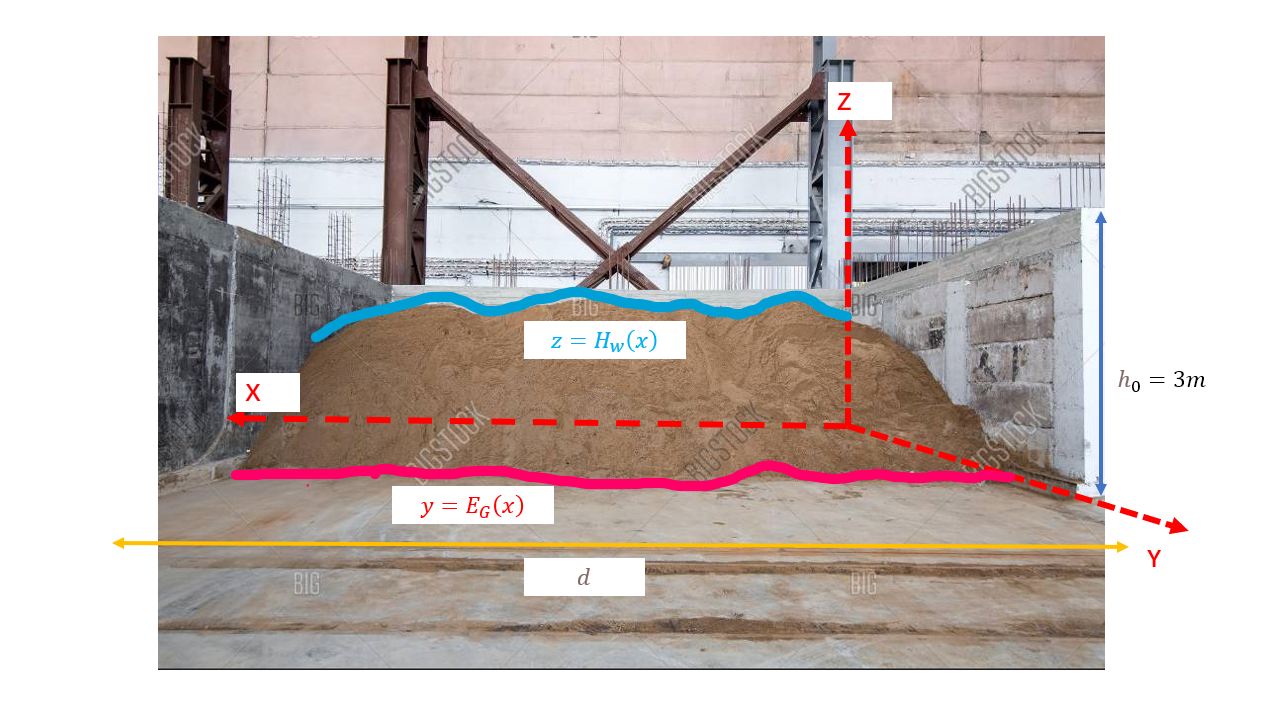
\includegraphics[width=\textwidth]{kuang_1.png}
    \caption{矿料仓库示意图} % 标题
    \label{kuang_1}
    \end {figure}

    首先我们需要指定摄像头在仓库中的位置。为了实时检测仓库的矿料体积,我们使用两个摄像头获取图像信息,上传至管理平台。两个摄像头分别位于仓库顶部以及仓库正面,分别拍摄仓库的俯视图与正视图。如图(\ref{camera_lay})中所示:

    \begin {figure}[h]
    \centering % 居中显示
    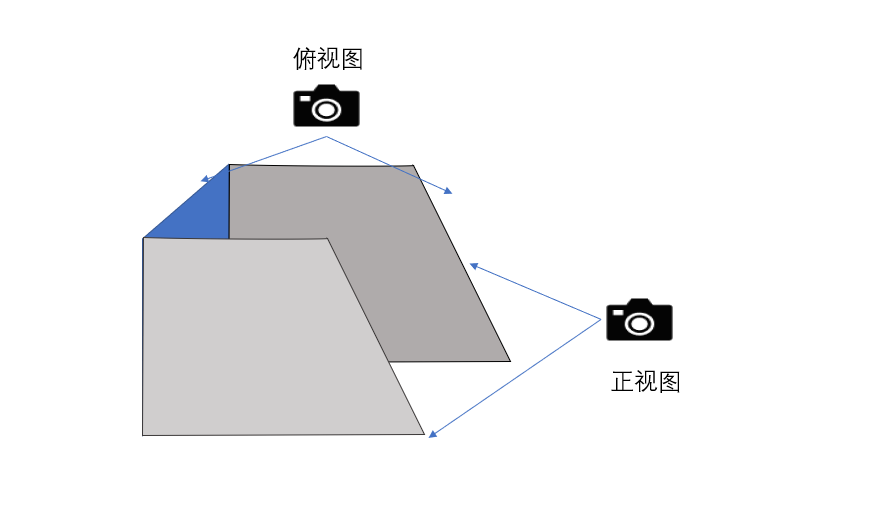
\includegraphics[width=\textwidth]{camera_lay.png}
    \caption{相机放置示意图} % 标题
    \label{camera_lay}
    \end {figure}

    在得到正视图以及俯视图后,我们需要进行边缘提取工作。边缘提取是计算机视觉领域较为成熟的一个领域,相当多边缘检测的算法被投入使用。考虑到现有条件下建立精确三维模型的困难之处,我们利用俯视图以及正视图中的边缘信息,还原矿料堆放的形状。从正视图中可以提取出矿料在后方墙体上的边缘投影$z=H_W(x)$,这有利于我们得到矿料整体高度。从俯视图中可以提取矿料的地面边缘信息$y=E_G(x)$。

    常见的的边缘检测算法\cite{bianyuan}有:使用Robort,Laplace,Sobel算子作为卷积核,在图像上进行滑动从而提取出边缘响应。此外还有若干基于模糊推理以及小波检测的方法,鉴于计算复杂性,我们采用Sobel算子(如图\ref{sobel})进行边缘信息提取。

    \begin {figure}[h]
    \centering % 居中显示
    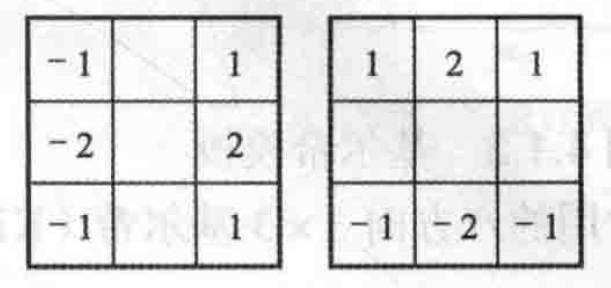
\includegraphics[width=0.5\textwidth]{sobel.png}
    \caption{sobel算子示意图} % 标题
    \label{sobel}
    \end {figure}

    在提取矿料边缘之后,我们将利用矿料地面边缘$E_G$,矿料墙体边缘$E_W$建立矿料体积模型。考虑到矿料位于四个平面之间,有两个面形状不规则,但利用矿料地面边缘$E_G$与墙壁信息可以计算出矿料的底面积大小,利用矿料墙体边缘$H_W$可以估计矿料堆放高度。再利用已知矿料的休止角$\theta$大小,可以建立以下体积计算公式:

    \begin{equation}
        V=0.5*\int_0^d H_W(x)*(2E_G(x)-\frac{H_W(x)}{tan(\theta)})
    \label{}
    \end{equation}

    ,其中$V$是矿料体积,x轴沿垂直于两面隔墙的方向,$\theta$是不同矿料的休止角。


    \subsubsection{堆放余量模型建立}
    
    我们首先考虑仓库中没有任何矿料的情况,此时$V=0$。在这一情况下,矿料装满后仓库侧视图如图(\ref{kuang_2} a)所示,此时$H_W(x)=h_0$且$E_G(x)=L_0$,$L_0$是仓库长度。

    在仓库不空的情况下,由于已有的矿料占据了仓库空间,使得已经堆放的矿料上方的空间得不到利用。此时仓库剩余体积$V_{remain}$不能使用总体积$V_0$与矿料体积$V$相减获得。此时剩余体积如图(\ref{kuang_2} b)中的红色部分所示.矿车在地面边缘$E_G$部分下料,填补原有矿料角度(部分1),在填平之后继续堆放高度至$h_0$,此时产生高低界面之间的斜坡(部分2),最终将仓库靠近出口处的剩余体积补齐(部分3),此时装填整个仓库。

    \begin{figure}[htbp]
        \centering  %居中
        \subfigure[仓库为空的剩余体积]{   %第一张子图
        \begin{minipage}{0.4\textwidth}%大小总和超过textwidth则自动换行
        \centering    %子图居中
        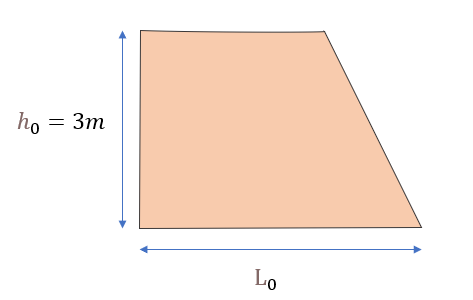
\includegraphics[width=\textwidth]{kuang_2_a.png}  %设置图片的输出大小倍数,这里是0.5倍大小输出
        \end{minipage}
        }
        \subfigure[仓库不空的剩余体积]{ %第二张子图
        \begin{minipage}{0.4\textwidth}
        \centering    %子图居中
        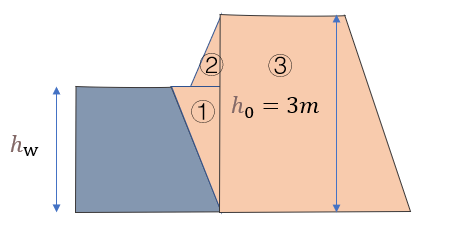
\includegraphics[width=\textwidth]{kuang_2_b.png}%以pic.jpg的0.5倍大小输出
        \end{minipage}
        }
        
    
        \caption{不同情况下的矿料剩余体积(侧视图)}    %大图名称
        \label{kuang_2}    %图片引用标记
    \end{figure}

    综合上述分析,我们提出矿料剩余体积计算公式:
        \begin{equation}
            V_{remain}=\begin{cases}V_0=0.5*d*h_0*(2L_0-\frac{h_0}{tan(\theta)}),仓库为空\\\frac{h_0^2}{2*tan\theta}+0.5*\int_0^d H_W(x)*(2(L_0-E_G(x))-\frac{h_0}{tan\theta})*
            \end{cases}
        \label{remain}
        \end{equation}

        \subsubsection{数量调配模型建立}
    
        我们利用矿料体积的估计结果,在不考虑矿料堆放形状的情况下,计算给定$V_{remain}$下所需要的车辆数$M$。

        \begin{equation}
            V_{remain}=V_{big}*M_{big}+V_{small}*M_{small}
        \end{equation}

        其中车子数量满足以下约束条件:
        \begin{equation*}
            0\leq M_{big} \leq M_{big,max}
        \end{equation*}
        \begin{equation*}
            0\leq M_{small} \leq M_{small,max}
        \end{equation*}

        ,$M_{max}$为最大车辆数目。

\subsubsection{模型的求解}
经过Sobel算子特征提取后,我们得到如图(\ref{sobel_r})所示的边缘响应:
,其中黄色部分为仓库中剩余矿料,黑色部分是仓库剩余面积。

\begin {figure}[h]
\centering % 居中显示
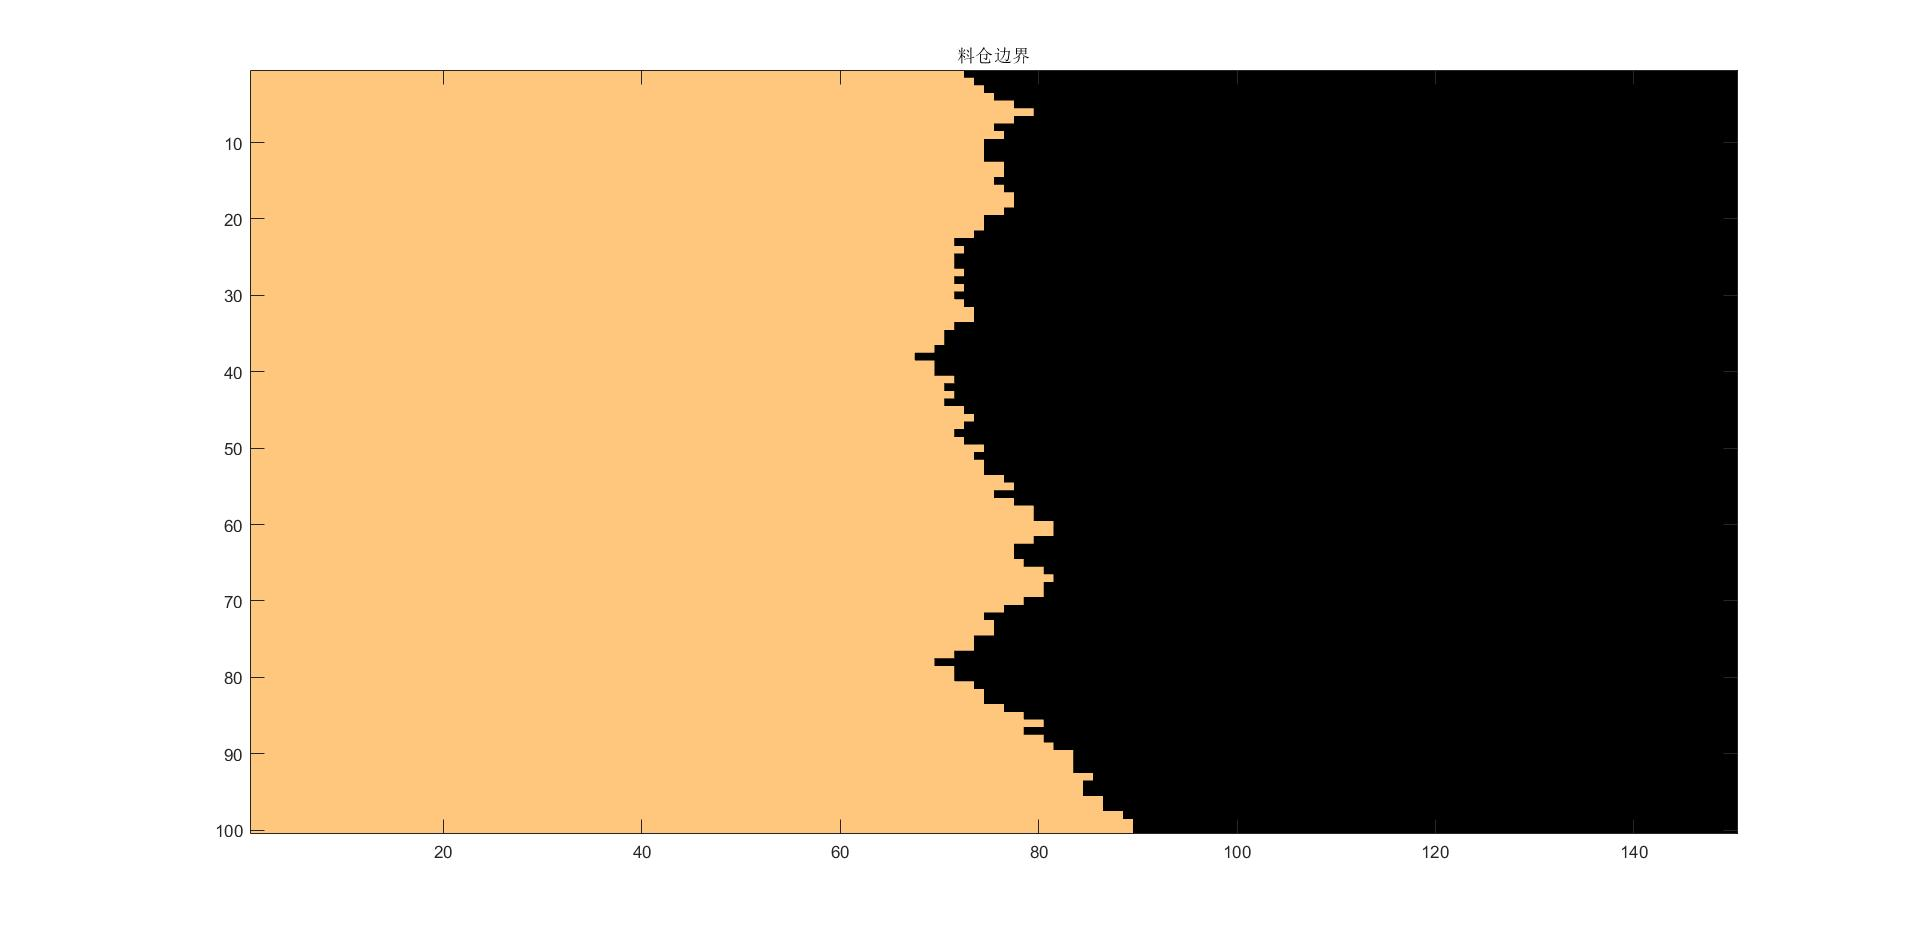
\includegraphics[width=\textwidth]{untitled.jpg}
\caption{地面边缘$E_G$结果} % 标题
\label{sobel_r}
\end {figure}

\subsection{问题二模型的建立与求解}
\subsubsection{矿料形态模型建立}
考虑自卸车卸下矿料的过程,在模型假设中,我们将自卸车看作是一个高度大于3米的漏斗。我们若是考虑矿料为刚性材料,那么卸下后形状不会发生变化,此时矿料形状为一个均匀的长方体,如图(\ref{heap})所示。事实上,考虑矿料的静止角等因素,该状态可以作为矿料堆放的初始状态。也就是说,在矿料倾倒下来的瞬间,矿料是长方体,在随后的一小段时间内遵循物理规律下落坍塌,形成坡面。

\begin {figure}[h]
\centering % 居中显示
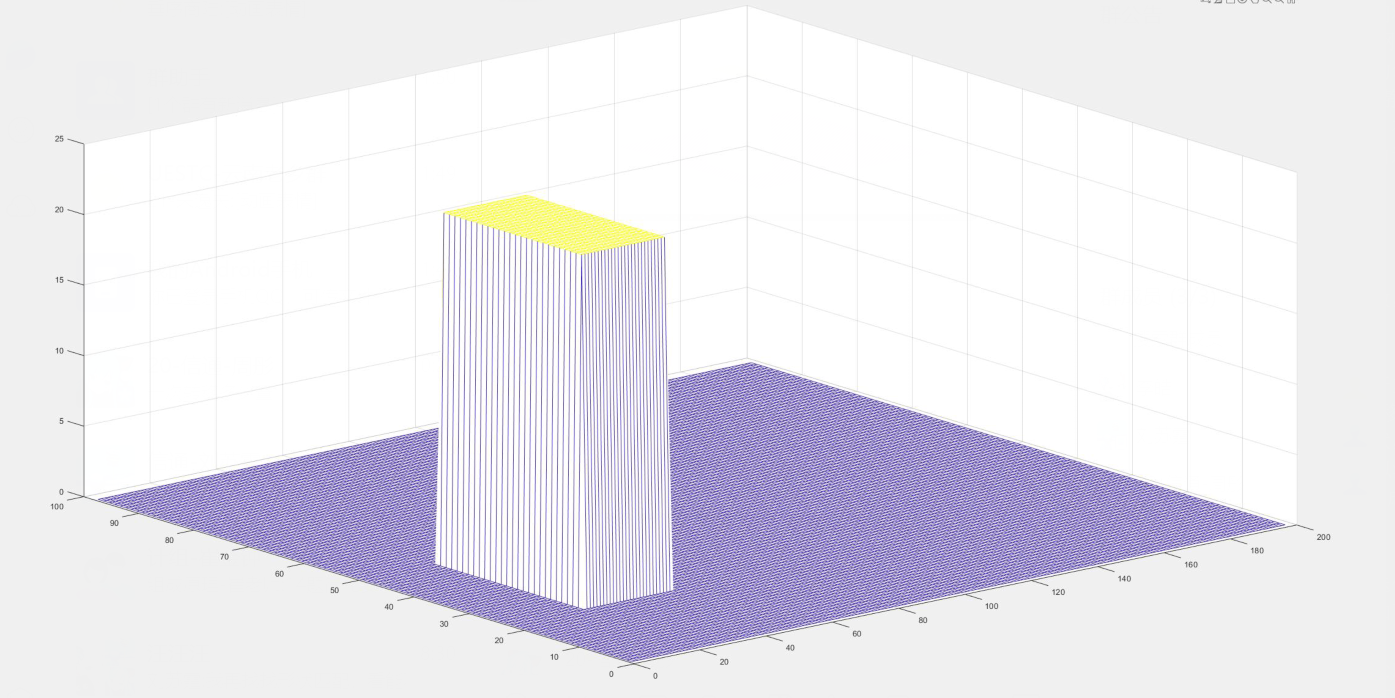
\includegraphics[width=\textwidth]{heap.png}
\caption{矿料堆放瞬间示意图} % 标题
\label{heap}
\end {figure}

该长方体的几何尺寸取决于大小自卸车的货厢参数,我们将在模型求解中给出具体尺寸。

前人在矿料等微粒集合体现出的宏观形状做出了许多研究,Yamakita\cite{waji}等人在使用挖掘机模型转移土壤的过程中,利用二维高斯函数拟合现实中沙子的堆放形状,Nuca\cite{paowuxian}等人提出退化的抛物线模型,对模拟沙子流动的行为做出了较好的建模,Song\cite{hesha}等人考虑了在河流冲刷外力作用的情况下沙子堆放形状问题。

在前人研究的启发之下,我们提出一种基于离散迭代的元胞自动机方法,建立矿料形状的物理模型。其理论基础如下:

矿料某点处的矿料稳定与否,取决于矿料在这点处的方向导数$\frac{\partial h}{\partial l}$与休止角正切值的大小关系$tan\theta$。若方向导数值大于休止角正切值,则该点不稳定,会发生坍塌。

\begin{equation}
    \frac{\partial h}{\partial l}\leq tan\theta
\end{equation}

我们定义坍塌为矿料不稳定点与相邻矿料点之间的物质转移情况。该转移过程中保持矿料体积不变,转移的方向沿该点高度值的负梯度方向。每次转移直到该点不会向周围再次滑动为止。而且在转移过程中需要保持矿料体积恒定,转移之后转移点不会比周围点都低。

我们对目前矿料上的每个点计算方向导数,按照方向导数从大到小的顺序进行坍塌结果计算。上述步骤称为一次形状迭代,形状迭代之后可能仍然不能使所有点都满足休止角的条件。因此迭代过程可能还需要再进行数次。

在迭代终止之后,我们便获得矿料堆放的最终形状。

考虑连续模型计算的困难性,我们结合元胞自动机的基本理论,提出离散的矿料物理模型。该模型将连续的矿料立方体网格化,将其分割为离散格点,格点上具有高度信息。我们利用格点高度矩阵$G$存储高度信息,如图(\ref{wangge}a)。对于每个格点,根据其周围格点的相对高度,具有以下行为特征:

\begin{figure}[htbp]
    \centering  %居中
    \subfigure[离散局部]{   %第一张子图
    \begin{minipage}{0.4\textwidth}%大小总和超过textwidth则自动换行
    \centering    %子图居中
    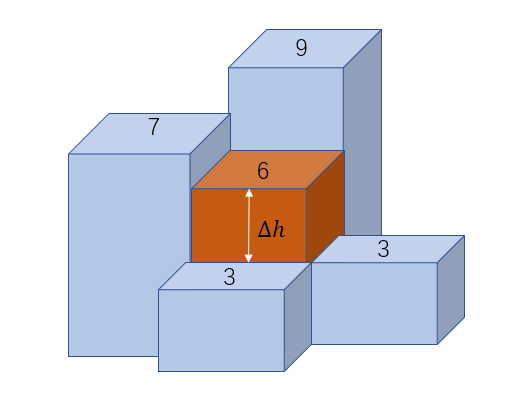
\includegraphics[width=\textwidth]{wangge_a.png}  %设置图片的输出大小倍数,这里是0.5倍大小输出
    \end{minipage}
    }
    \subfigure[网格矩阵示意图$H$]{ %第二张子图
    \begin{minipage}{0.4\textwidth}
    \centering    %子图居中
    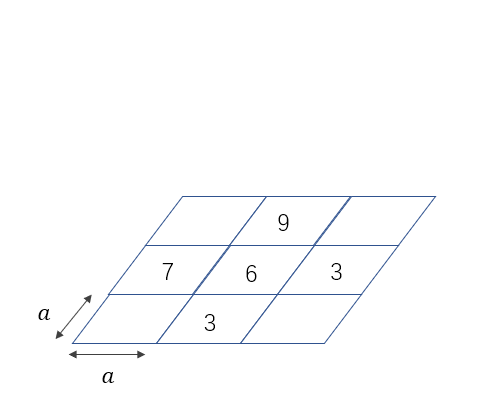
\includegraphics[width=\textwidth]{wangge_b.png}%以pic.jpg的0.5倍大小输出
    \end{minipage}
    }

    \caption{离散矿料模型示意图}    %大图名称
    \label{wangge}    %图片引用标记
\end{figure}

离散化梯度计算,使用差分代替求导。某个格点$V_0$在各个方向的梯度使用各个方向上的高度差$\Delta h$与网格边长$a$之比计算,我们称之为离散梯度$p$格点是否发生坍塌,依然取决于下式:

\begin{equation}
    p=\frac{\Delta h}{a}\leq tan\theta
\label{}
\end{equation}

在网格边界处设置边界高度为无穷,此时离散梯度$\frac{\Delta h}{a}$恒小于休止角$tan\theta$,也就是不会坍塌至边界以外。

考虑到元胞自动机的有限行为特点,坍塌时候发生物质转移只在当前网格的四邻域方向进行。基于当前点和周围点的高度信息,我们可以计算并记录四个方向的离散梯度,我们使用梯度数组$P$维护:

\begin{equation}
    P=[\frac{\Delta h_{up}}{a},\frac{\Delta h_{down}}{a},\frac{\Delta h_{left}}{a},\frac{\Delta h_{right}}{a}]
\end{equation}

我们对每个方向上的离散梯度$p$与休止角正切值$tan\theta$比较,得到坍塌方向数$N$:

\begin{equation}
    N=|\{p|p>tan\theta,p\in P\}|
\end{equation}

若梯度数组中数值都小于休止角正切值$tan\theta$,也就是$N=0$的情况下,该点不发生坍塌。下面重点讨论$1 \leq N$的情况:

此时约束条件有以下三条:
\begin{enumerate}
    \item 当前格点处可能向周围不满足休止角的方向进行坍塌,坍塌至$p<tan\theta$。
    \item 每个方向上都可能发生坍塌,且当前格点$V_0$的高度$h_{v0}$不会因为坍塌而低于周围格点。
    \item 当前格点以及周围格点的高度之和不会发生改变,这是因为物质守恒原理。
\end{enumerate}

在上述约束条件下,我们得到高度更新公式:
\begin{equation}
    h_{v0} + a*\sum p =h^*_{v0}+N^*(h^*_{v0}-tan\theta)
\end{equation}
\begin{equation}
    h* = h_{v0}^* -tan\theta
\end{equation}

,其中$h_{v0}^*$代表坍塌后当前网格点的高度。

\subsubsection{调度策略模型建立}

为了使仓库装载矿料尽可能多,我们需要实时计算最佳的卸货位置以及最佳的卸货车型,以实现最终堆放的体积最大。因为我们是在已有部分矿料的仓库中中继续填,在自卸车加入新的矿料之后,形成的形状并不是对应点高度的简单相加。也就是说每次卸料的结果都与当前仓库矿料的堆放状态有关。

同时我们发现,仓库的界限(如地面、隔墙等)是平整的,且不能有矿料溢出。加之矿料堆放的物理模型中,我们规定矿料堆放到$h_0$,也就是仓库隔墙的高度。所以只要保证每次卸货的结果都尽量维持地面边缘的平整,那么最后就可以使得仓库装料体积最大。

下面介绍如何选择最佳卸货位置。在矿料体积模型中,我们采用计算机视觉方法提取矿料的地面边缘$E_G$。在矿料物理模型中我们已将靠墙情况下的自卸车在平地上的堆放结果(如图\ref{chedui})模拟出来。我们将这一堆放结果轮廓称为$S$。

chedui 平地上靠墙的的堆放结果

向已经堆放矿料的仓库中卸货时,“漏斗”边缘位置受到原有矿料的影响,只能在矿料的地面边缘的一段距离$d$之内,如图(\ref{kuangbian}),也就是说自卸车能够深入仓库的距离是有限的。

\begin {figure}[h]
\centering % 居中显示
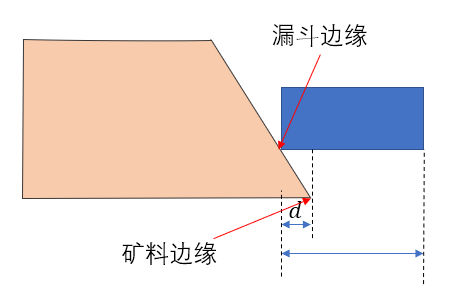
\includegraphics[width=0.6\textwidth]{kuangbian.png}
\caption{漏斗边缘和矿料边缘的位置示意图} % 标题
\label{kuangbian}
\end {figure}

为了计算极限距离$d$,我们需要考虑自卸车的离去角$\alpha$与休止角$\theta$之间的关系。车辆的离去角定义为车满载时自车身后端突出点向后车轮引切线与路面之间的夹角\cite{liqu}。
主要分为两种情况,如图(\ref{liqu}):
\begin{itemize}
    \item 小自卸车离去角$\alpha_{small}$较小、小于矿料的安息角时,卸货的深度只受物料安息角车和货箱最低点的高度影响,这是小型自卸车的情况。
    \item 大自卸车的离去角$\alpha_{big}$较大,轮子会先触碰到矿料,而货箱不会触碰矿料。
\end{itemize}

\begin{figure}[htbp]
    \centering  %居中
    \subfigure[小装卸车离去角$\alpha$与休止角$\theta_{f,c}$示意图]{   %第一张子图
    \begin{minipage}{0.4\textwidth}%大小总和超过textwidth则自动换行
    \centering    %子图居中
    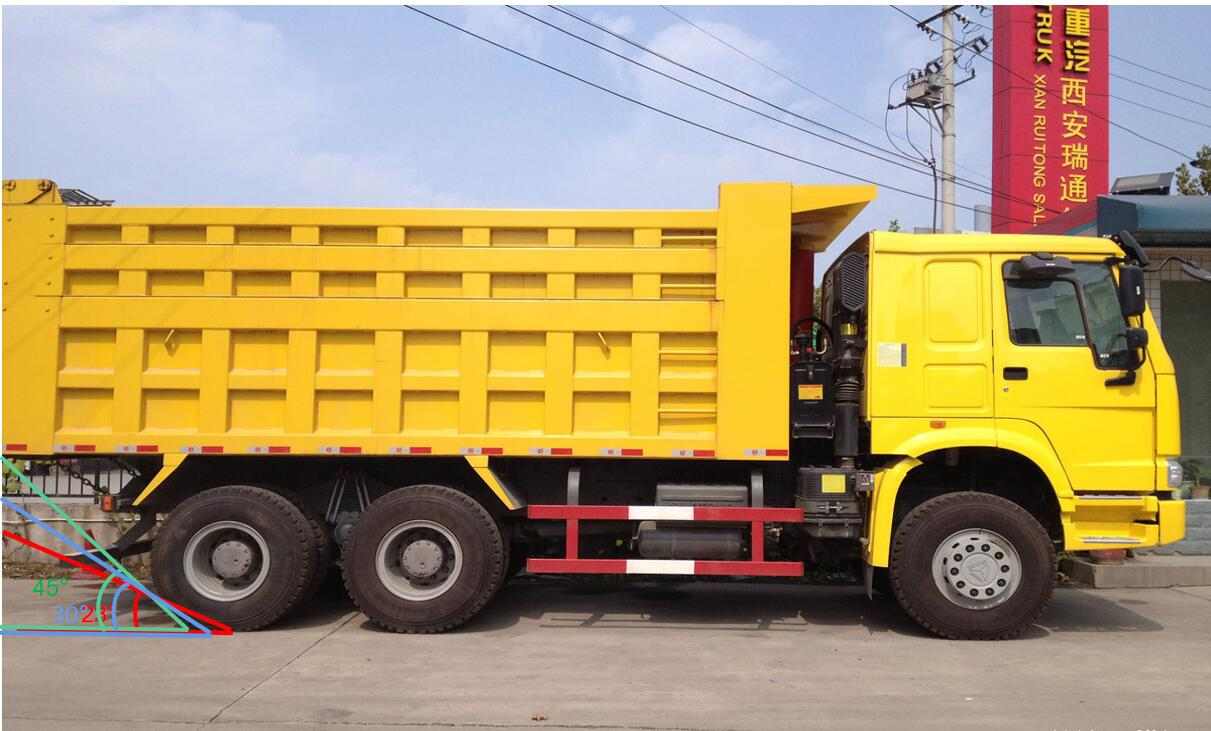
\includegraphics[width=\textwidth]{liqu_a.jpg}  %设置图片的输出大小倍数,这里是0.5倍大小输出
    \end{minipage}
    }
    \subfigure[大装卸车离去角示意图]{ %第二张子图
    \begin{minipage}{0.4\textwidth}
    \centering    %子图居中
    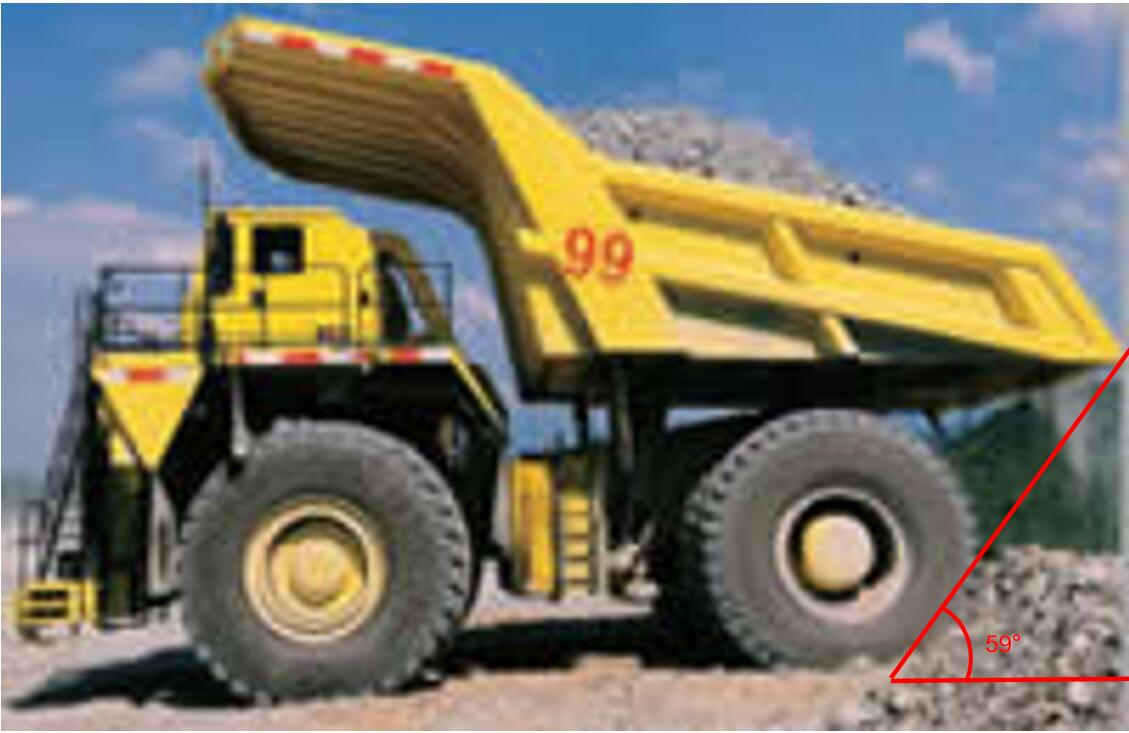
\includegraphics[width=\textwidth]{liqu_B.jpg}%以pic.jpg的0.5倍大小输出
    \end{minipage}
    }

    \caption{自卸车离去角示意图}    %大图名称
    \label{liqu}    %图片引用标记
\end{figure}

经查阅资料\cite{che_1,che_2},小车的货箱最低点高度$h_{small} = 0.98m$ ,离去角$\alpha_{small} =23\deg$,细矿砂休止角$\theta_{f}=30\deg$,所以小型自卸车货箱边界能够深入已有细矿料边界的距离为:

\begin{equation*}
    d_{small,f} = \frac{h_{small}}{tan\theta_{f}}=1.66m
\end{equation*}

;对于粗砂,其安息角更大,同理可以计算得到:
\begin{equation*}
    d_{small,c} = \frac{h_{small}}{tan\theta_{c}}=0.98m
\end{equation*}

对于大自卸车而言,无论是粗料还是细料都达不到离去角,因此$d_{big}$使用下式进行计算:

\begin{equation*}
    d_{big} = \frac{H_{big}}{tan\alpha_{big}}
\end{equation*}

,记算得到$d_{big}=1.09m$。

虽然矿料的堆放是一个三维立体模型,但是因为假设1中,已有矿料的角度统一为安息角,且边界基本规整。因此我们可以将此三维模型抽象成一个二维模型,即只考虑其俯视图,只考虑边界的形状。我们用第一问靠墙堆放情况下的坍塌模型得到的边界为匹配目标,因为虽然不同情况下重叠堆放出来的堆的形状会发生变化,但因为卸货车卸货深度的限制,其最终结果应与靠墙堆放相似。

在确定大小车辆在不同矿料条件下的极限距离$d$之后,我们使用边界相似的方法最佳位置。该方法首先将已有矿料的地面边缘$E_G$分为等距网格下的100个点为采样点,为了计算边界相似度。从第一问的靠墙坍塌情况下模拟会得到一个边界图(图\ref{qiangdui}b),我们以此为目标形状的外边界$S$,在距离外边界卸货车深入矿物的最大距离$d$处记录内部边界$S’$内外边界之间形成模板,我们在等距网格上移动这一模板,并且保持内边界紧贴已有矿料地面边缘$E_G$,并且使外边界在仓库出口边界以内,不断移动模板,这样我们会得到100个模板响应$R_i$。

\begin {figure}[h]
\centering % 居中显示
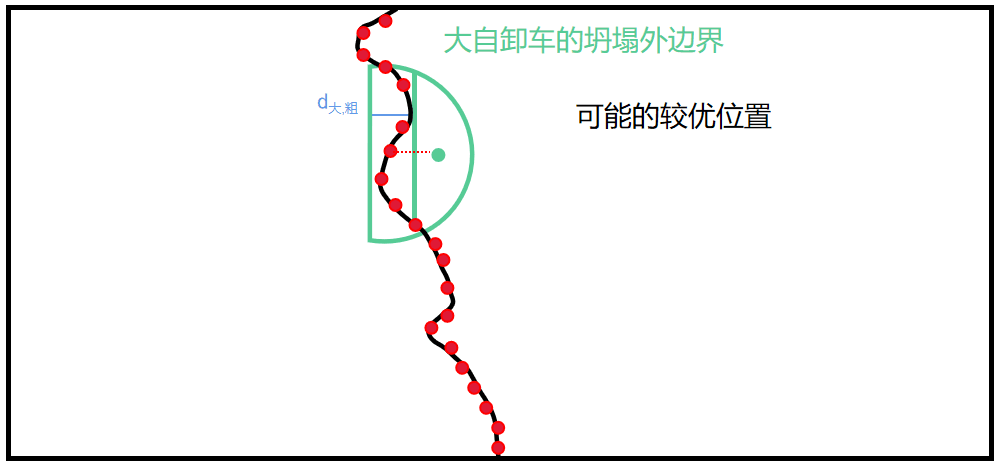
\includegraphics[width=\textwidth]{neiwai.png}
\caption{内外边界$SS'$示意图(绿色)} % 标题
\label{neiwai}
\end {figure}

模板响应$R$的计算方法为:计算目标图形在每次移动中的内外边界$SS’$所围区域内原有矿料含有地面边缘$E_G$采样点的个数$n$,与轮廓的周长$c(S)$的比值,作为边界相似度的度量。计算公式为:

\begin{equation*}
    R_{i,k}=\frac{n}{c(S)}
\end{equation*}

最后得到200个响应值$R$,大车、小车各100个,我们以$R$值最大的测试点位置为最佳位置$D$,同时以其需要的车型号为此位置对应的最佳车型$CN$。

\subsection{模型求解}

当大车和小车装载不同矿料时,在没有任何约束的平地上堆放情况如图(\ref{ping_dui})所示:

\begin{figure}[htbp]
    \centering  %居中
    \subfigure[粗料]{   %第一张子图
    \begin{minipage}{0.6\textwidth}%大小总和超过textwidth则自动换行
    \centering    %子图居中
    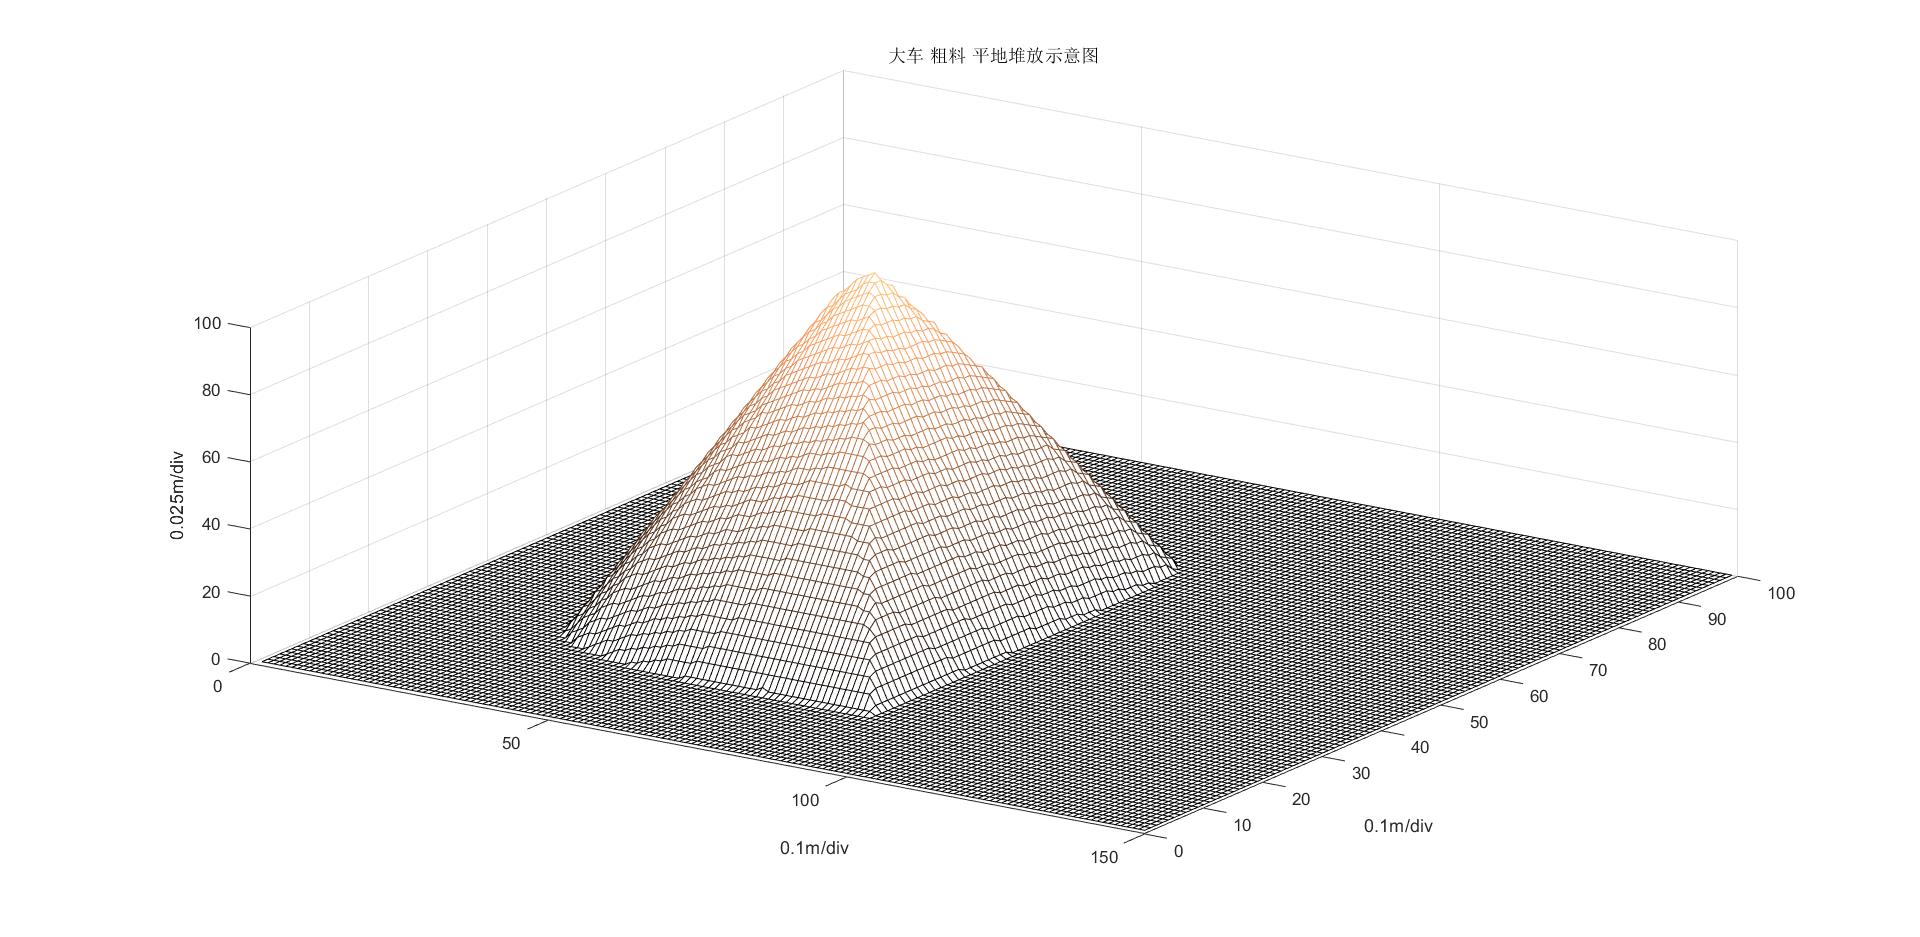
\includegraphics[width=\textwidth]{ping_dui_c.jpg}  %设置图片的输出大小倍数,这里是0.5倍大小输出
    \end{minipage}
    }
    \subfigure[细料]{ %第二张子图
    \begin{minipage}{0.6\textwidth}
    \centering    %子图居中
    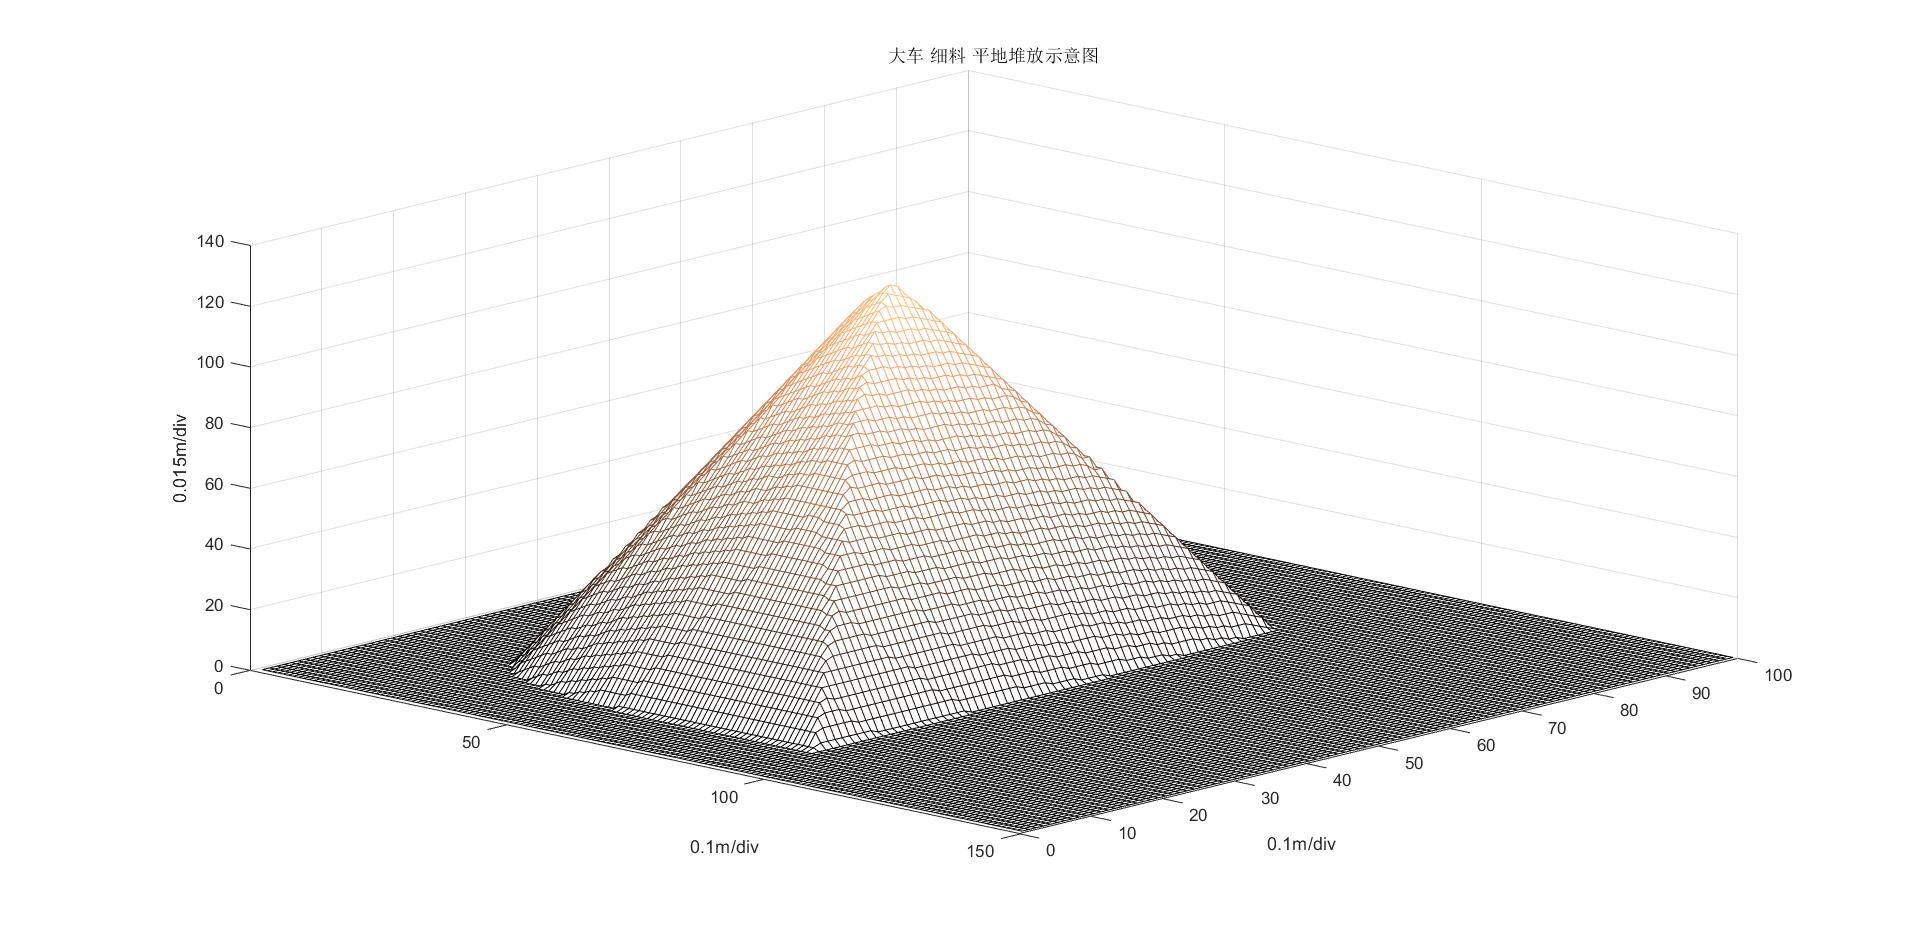
\includegraphics[width=\textwidth]{ping_dui_f.jpg}%以pic.jpg的0.5倍大小输出
    \end{minipage}
    }
    \caption{大车在水平地面堆放不同矿料示意图}    %大图名称
    \label{ping_dui}    %图片引用标记
\end{figure}

可见粗料由于其较大的静止角$\theta$,最终堆放高度较高。

当大车和小车搭载不同矿料时,在一侧靠墙的堆放情况如图(\ref{qiangdui})所示:
\begin{figure}[htbp]
    \centering  %居中
    \subfigure[三维视图]{   %第一张子图
    \begin{minipage}{0.6\textwidth}%大小总和超过textwidth则自动换行
    \centering    %子图居中
    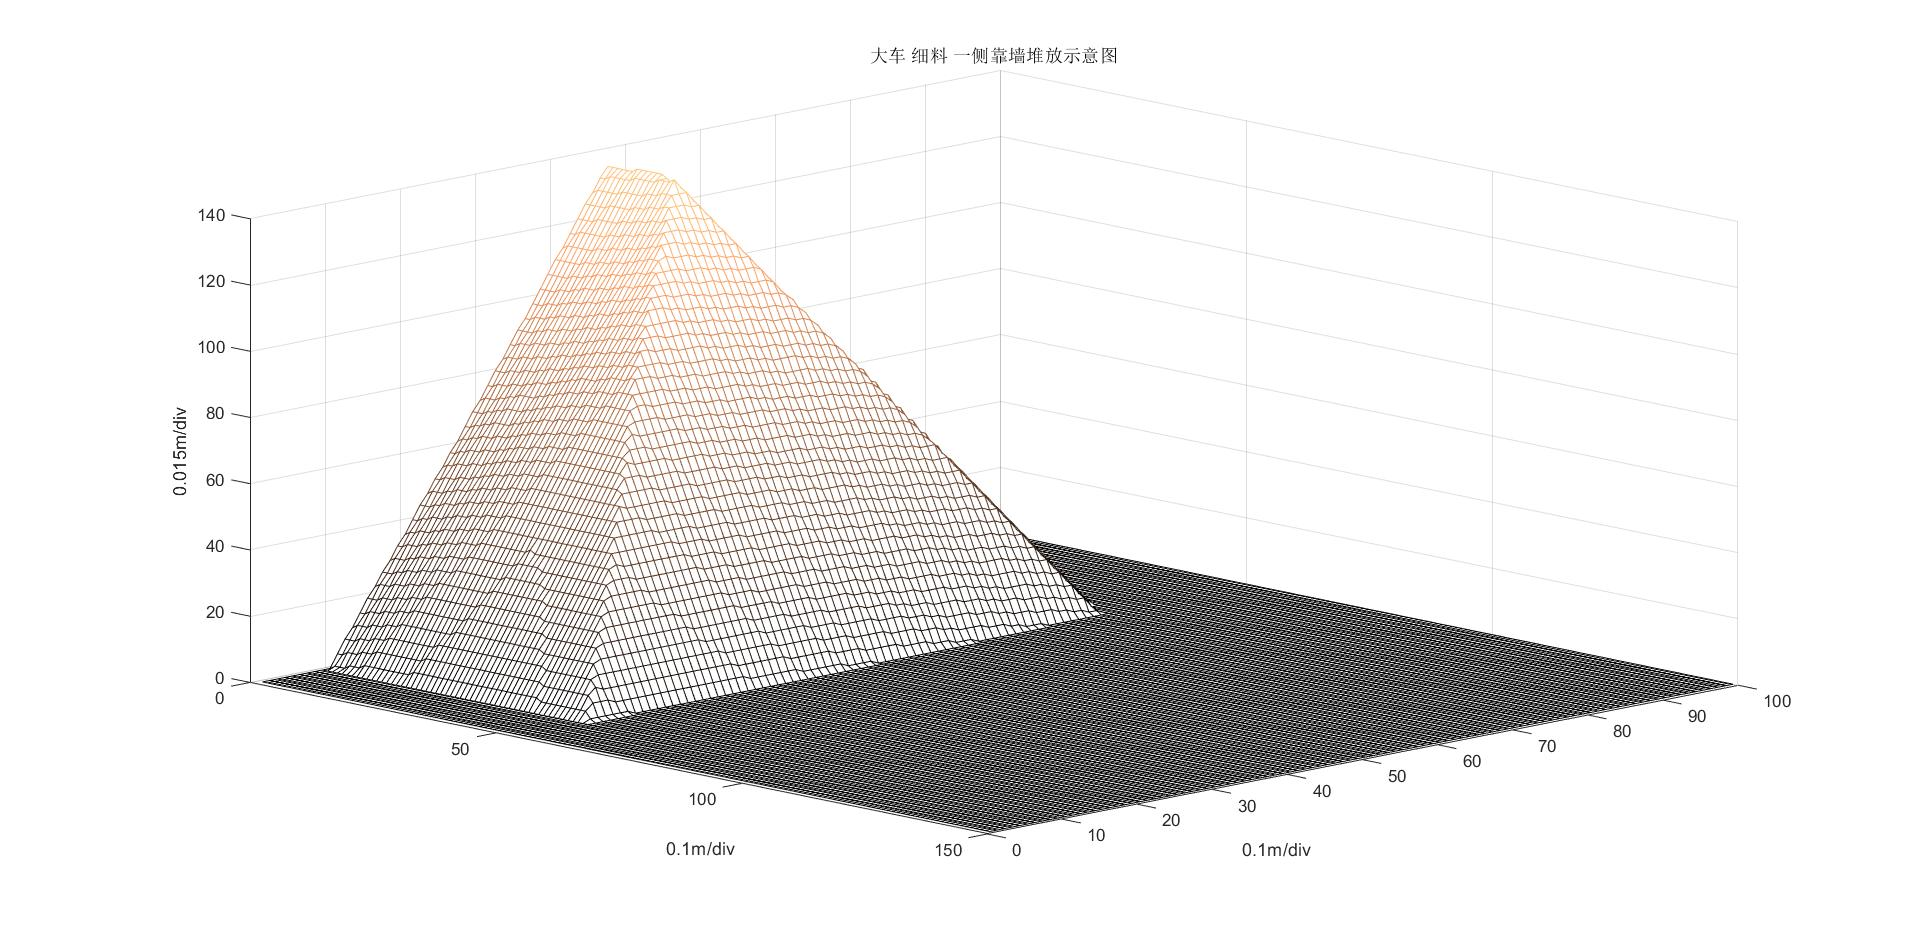
\includegraphics[width=\textwidth]{qiangdui_3.jpg}  %设置图片的输出大小倍数,这里是0.5倍大小输出
    \end{minipage}
    }
    \subfigure[俯视图]{ %第二张子图
    \begin{minipage}{0.6\textwidth}
    \centering    %子图居中
    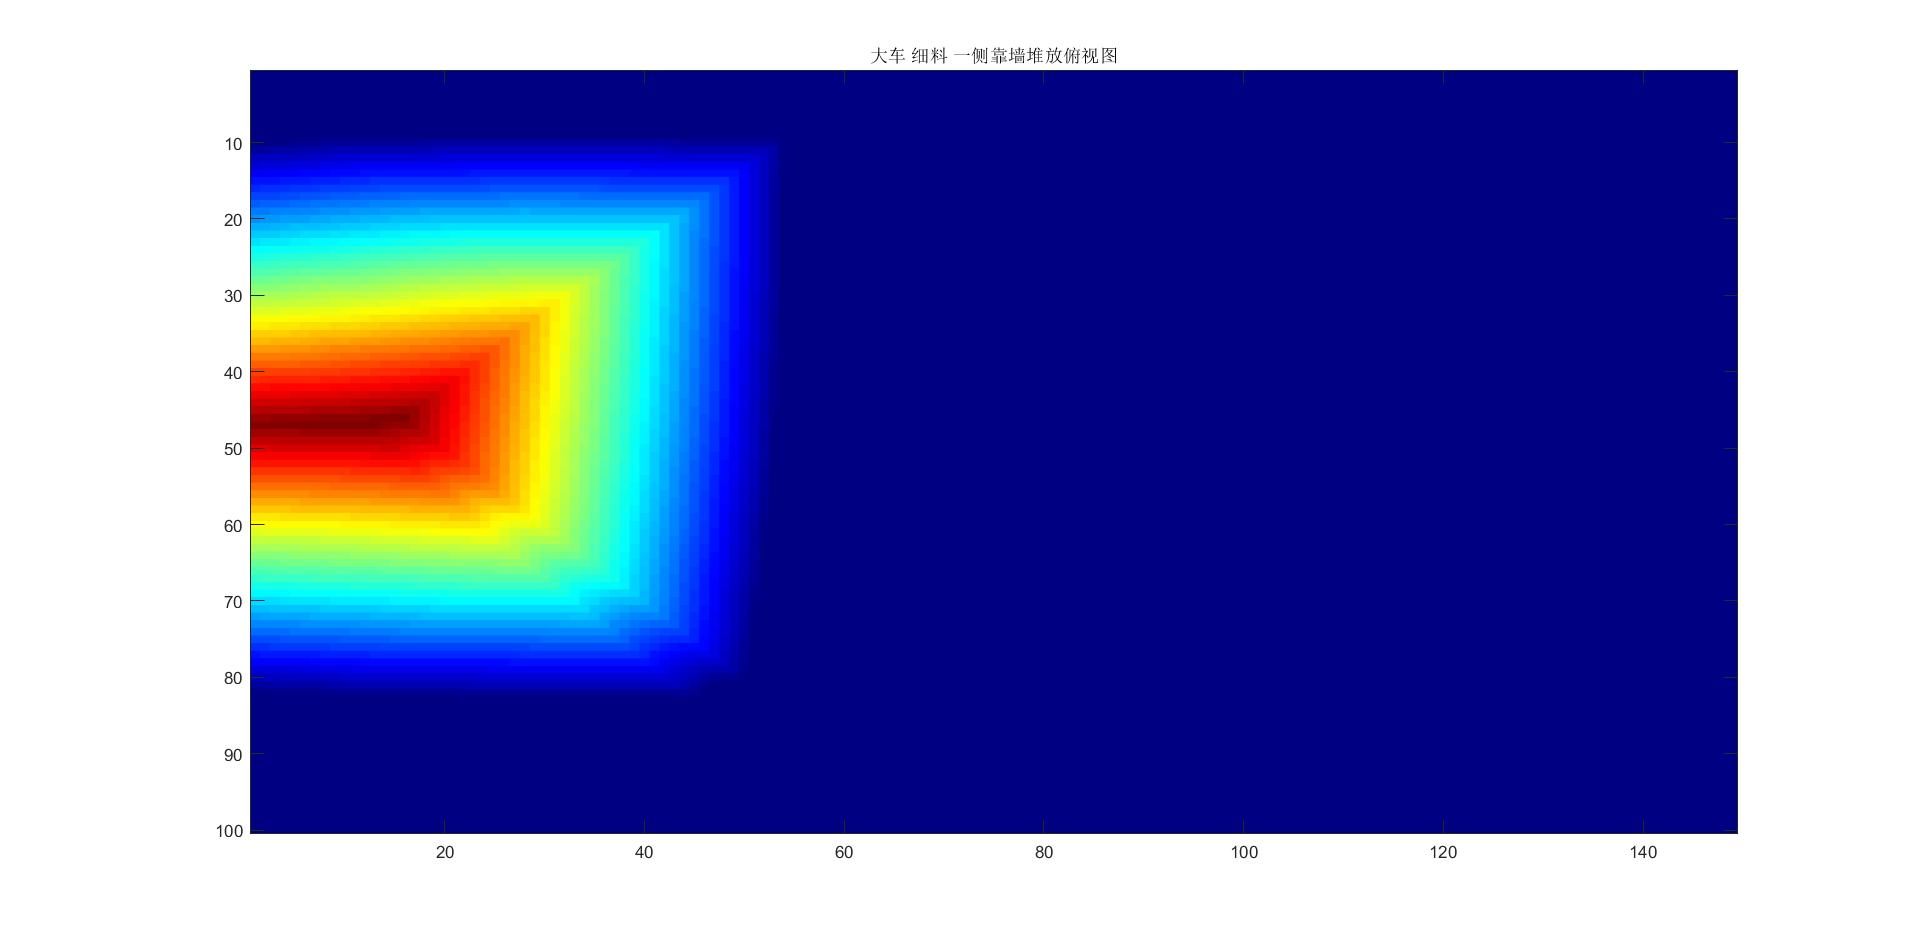
\includegraphics[width=\textwidth]{qiangdui_fu.jpg}%以pic.jpg的0.5倍大小输出
    \end{minipage}
    }

    \caption{大车细料在一侧靠墙的水平面上堆放示意图}    %大图名称
    \label{qiangdui}    %图片引用标记
\end{figure}

\subsection{问题三模型的建立与求解}

\subsubsection{仓库优先填充模型}

第二问中我们已经可以求出每个仓库最需要的自卸车类型$CN$和位置$D$。在第三问中,我们建立对于$M=6$个仓库的矿料调度问题:我们先求出各个仓库最需要的自卸车类型$CN_m$($m$为仓库序号)及最佳位置$P_m$($m$为仓库的编号,$i$为测试点的序号),然后优先满足编号较小的仓库对自卸车类型的需要。那么每个仓库的实际所装备的自卸车种类$C_m$指派规则如下:

考虑到需要使每个仓库都尽可能堆放较多的矿料,所以我们采取第二问中对每个仓库某时刻的最佳车型、位置的选择模型;但又要在大小自卸车仅各有一辆的情况下优先编号较小的仓库,所以我们增加了优先级模型。即如果多个仓库同时需要同一种类型的自卸车,我们优先满足编号小的需求,同时拒绝其余对此型号车的需求。及让其等待,直到编号比其小的所有仓库都不再对此类型车有需求,我们再为其分配此车。自卸车型号分配好后,其具体在某仓库的卸货位置,就是对应仓库计算出的$P_m$。

\section{七、模型的评价}

\subsection{模型的优点}
\begin{enumerate}
    \item 采用两个普通摄像头确定仓库中剩余矿料的体积,计算简便,成本低廉,且采用成熟算法响应速度快。

    \item 利用元胞自动机理论模拟矿料的坍塌过程,采用离散化思想,简化运算,计算速度快,易于实时模拟堆料过程的最优方案。
    
    \item 利用形状匹配的方法确定在何处堆料,利用三维仓库信息图的二维投影确定位置,计算准确度高,适应迭代过程。
\end{enumerate}

\subsection{模型的缺点}
\begin{itemize}
    \item 利用较少视觉信息估计仓库体积,效果不稳定,对矿料和背景的对比度较低的情况下识别准确率不高。
\end{itemize}

%----------- 参考文献 ----------
\newpage
\bibliographystyle{unsrt} %规定了参考文献的格式
\begin{center}
\bibliography{reference} %调出LaTeX生成参考文献列表
\end{center}

%----------- 附录 ----------
\newpage
\section{附录}

\textbf{sobel边缘检测代码}
\begin{lstlisting}[language=python]
    import logging
format ="%(asctime)s.%(msecs)05d : %(message)s"
logging.basicConfig(format=format,level=logging.INFO,datefmt="%H:%M:%S")

from PIL import Image
from numpy import asarray
import numpy as np
import math

def mask_slid_for_3x3 (img,mask_x,mask_y,thershold=140,file_name='pic'):
    (x_length, y_length) = img.shape
    img_x = img.astype('int32')
    img_y = img.astype('int32')
    img_g_1 = img.astype('int32')
    img_g_2 = img.astype('int32')
    img_g_i = img.astype('int32')
    #   复制备份
    padding_img = np.pad(img, ((1, 1), (1, 1)), 'edge').astype('int32')
    #     使用复制填充边缘
    for i in range(x_length):
        for j in range(y_length):
            block = padding_img[i:i + 3, j:j + 3]
            temp_x = block * mask_x
            temp_y = block * mask_y
            temp_x = temp_x.sum()
            temp_y = temp_y.sum()
            img_x[i][j] = temp_x
            img_y[i][j] = temp_y
            img_g_1[i][j] = abs(temp_x)+abs(temp_y)
            img_g_2[i][j] = math.sqrt(temp_x**2+temp_y**2)
            img_g_i[i][j] = max(temp_y,temp_x)

    single_dir_pic = [img_x,img_y]
    for i,img_copy in enumerate(single_dir_pic):
        sub_img = img_copy - img
        sub_img -= sub_img.min()
        sub_img = sub_img.astype('float64')
        sub_img *= (255.0 / sub_img.max())
        sub_img = sub_img.astype('uint8')
        im = Image.fromarray(sub_img)
        im.save(fp= file_name + str(i)+ '.png',
                format='png')

    grad_pic =[img_g_1,img_g_2,img_g_i]
    for i, img_copy in enumerate(grad_pic):
        sub_img = img_copy - img
        sub_img -= sub_img.min()
        sub_img = sub_img.astype('float64')
        sub_img *= (255.0 / sub_img.max())
        sub_img = sub_img.astype('uint8')
        sub_img_b = np.where(sub_img > thershold, 255, 0)
        im_b = Image.fromarray(sub_img_b.astype('uint8'))
        im_b.save(fp= + file_name+str(i+2) + 'b.png',
                  format='png')
    logging.info("finished !")

pil_im = Image.open("sky.png").convert('L')
im_array = asarray(pil_im)

Sobel_mask_x = np.array([[-1,0,1],
                         [-2,0,2],
                         [-1,0,1]])

Sobel_mask_y = np.array([[1,2,1],
                         [0,0,0],
                         [-1,-2,-1]])


mask_slid_for_3x3(im_array,Sobel_mask_x,Sobel_mask_y,thershold=110,file_name='sky_sobel_110_')



\end{lstlisting}




\end{document}